\documentclass[report]{BetterDocument}

\newcommand{\ofc}{Open Food Facts}
\newcommand{\bdd}{base de données}

\title{Buy Or Not}
\subtitle{Doc Utilisateur}
\who{MARTIN Justine}
\date{}
\place{BTS SIO 2 - Jean Rostand Caen}

\begin{document}

	\pageDeGarde

	\tableDesMatieres

	\chapter{Présentation}

	La présente application Android a pour but la gestion des produits en utilisant une \bdd{} semblable à celle d'\ofc{}. En effet, si cette application est satisfaisante, on pourra alors la redévelopper en utilisant cette fois ci la \bdd{} d'\ofc{} tout en s'appuyant sur le code préexistant. Cette documentation a donc pour objectif de présenter le fonctionnement de l'application pour les utilisateurs afin de les accompagner dans la prise en main de celle ci.

	Attention, toutes les fonctionnalités ne sont pas implémentées. L'objectif principal de l'application est respecté cependant des informations comme le pays de provenance, les catégories, etc sont volontairement omises, l'application n'étant actuellement conçue que dans un cadre d'ébauche pour un éventuel développement à plus grande échelle.

	\chapter{Gestion des produits}
	\section{Lister les produits}

	Lorsque vous démarrez l'application, vous arrivez automatiquement sur l'écran qui permet de visualiser l'ensemble des produits disponibles dans la \bdd{}. Par défault il s'agit de l'ordre dans lequel les produits ont été ajoutés. Le plus récent est au sommet de celle liste et les plus anciens au plus bas de celle ci.

	\begin{figure}[H]
		\centering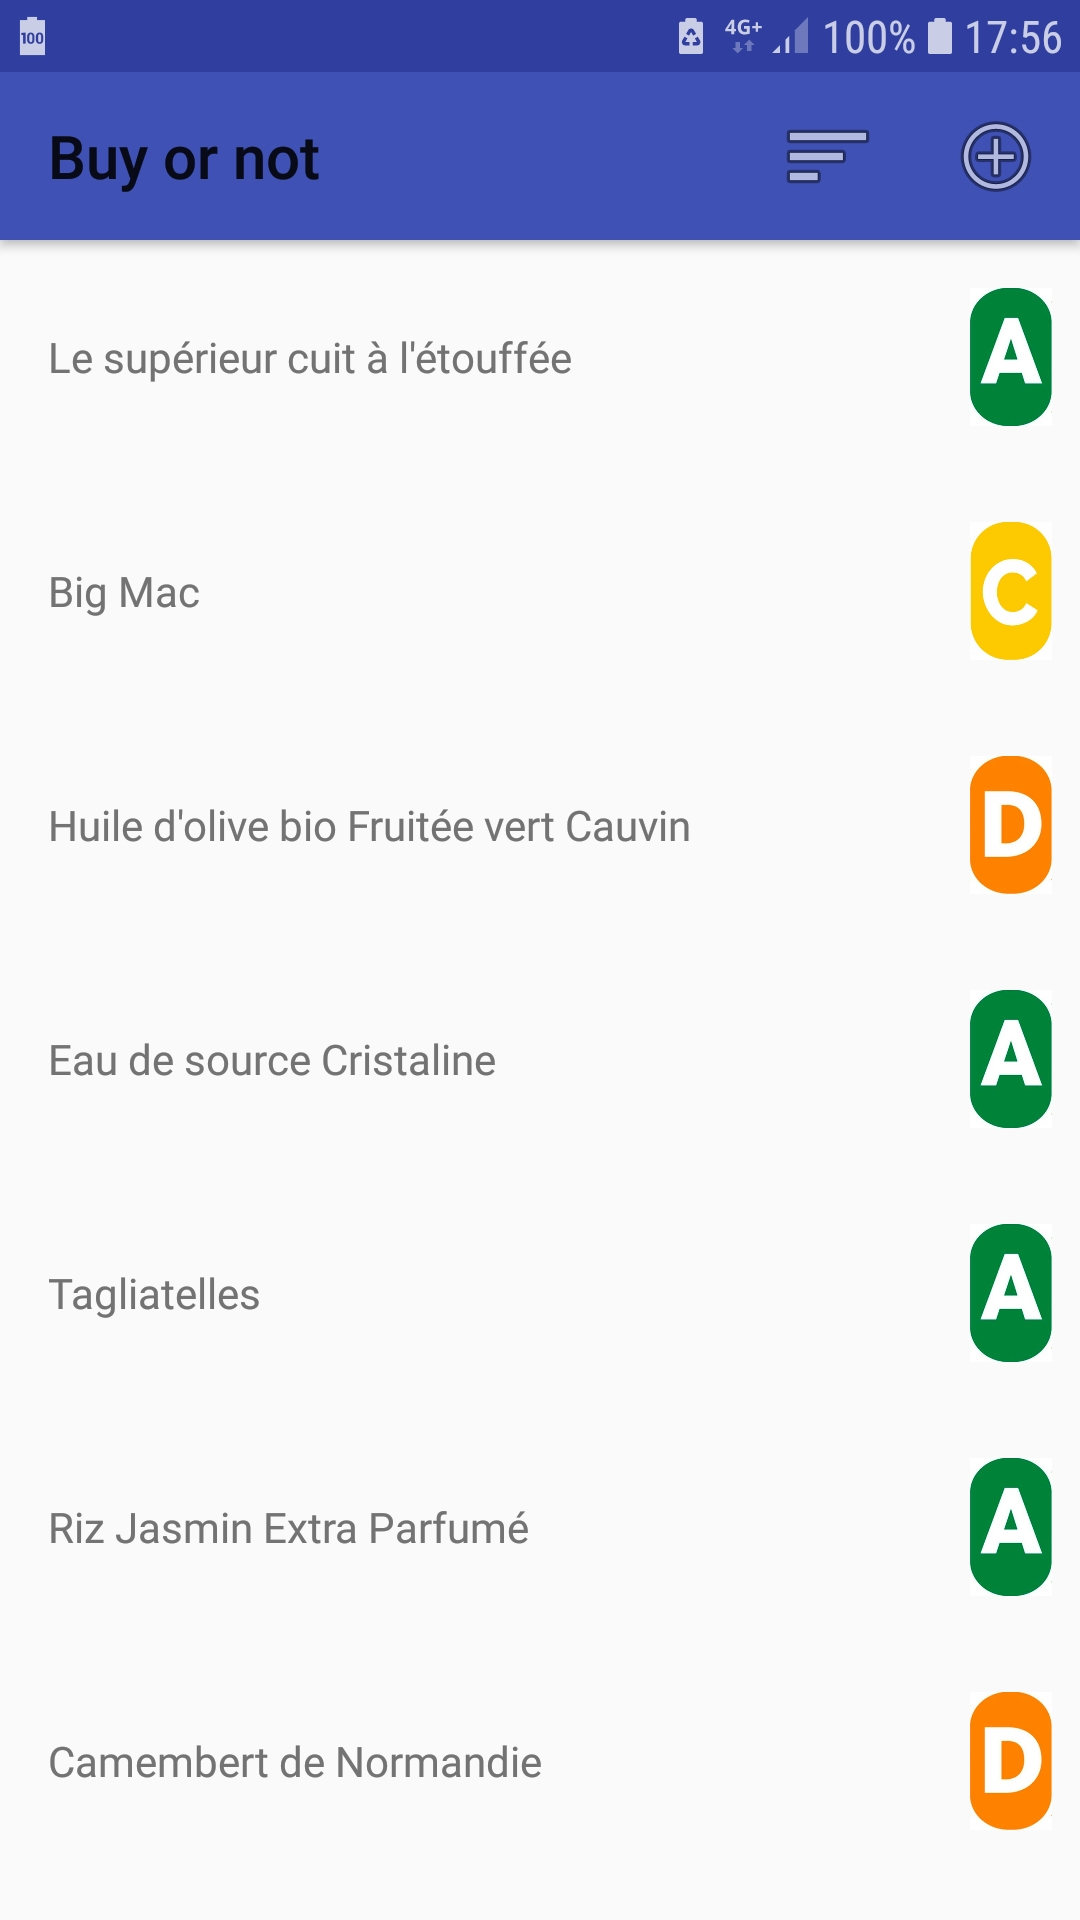
\includegraphics[width=0.5\paperwidth, height=0.3\paperheight, keepaspectratio]{img/lister_recent.jpg}
		\captionof{figure}{Listing des produits par ordre d'ajout}
		\label{produit:consulter}
	\end{figure}

	Le bouton en haut à gauche nous permet de sélectionner la méthode de tri que l'on souhaite. Ainsi il est possible de sélectionner un mode parmis les suivants :

	\begin{figure}[H]
		\centering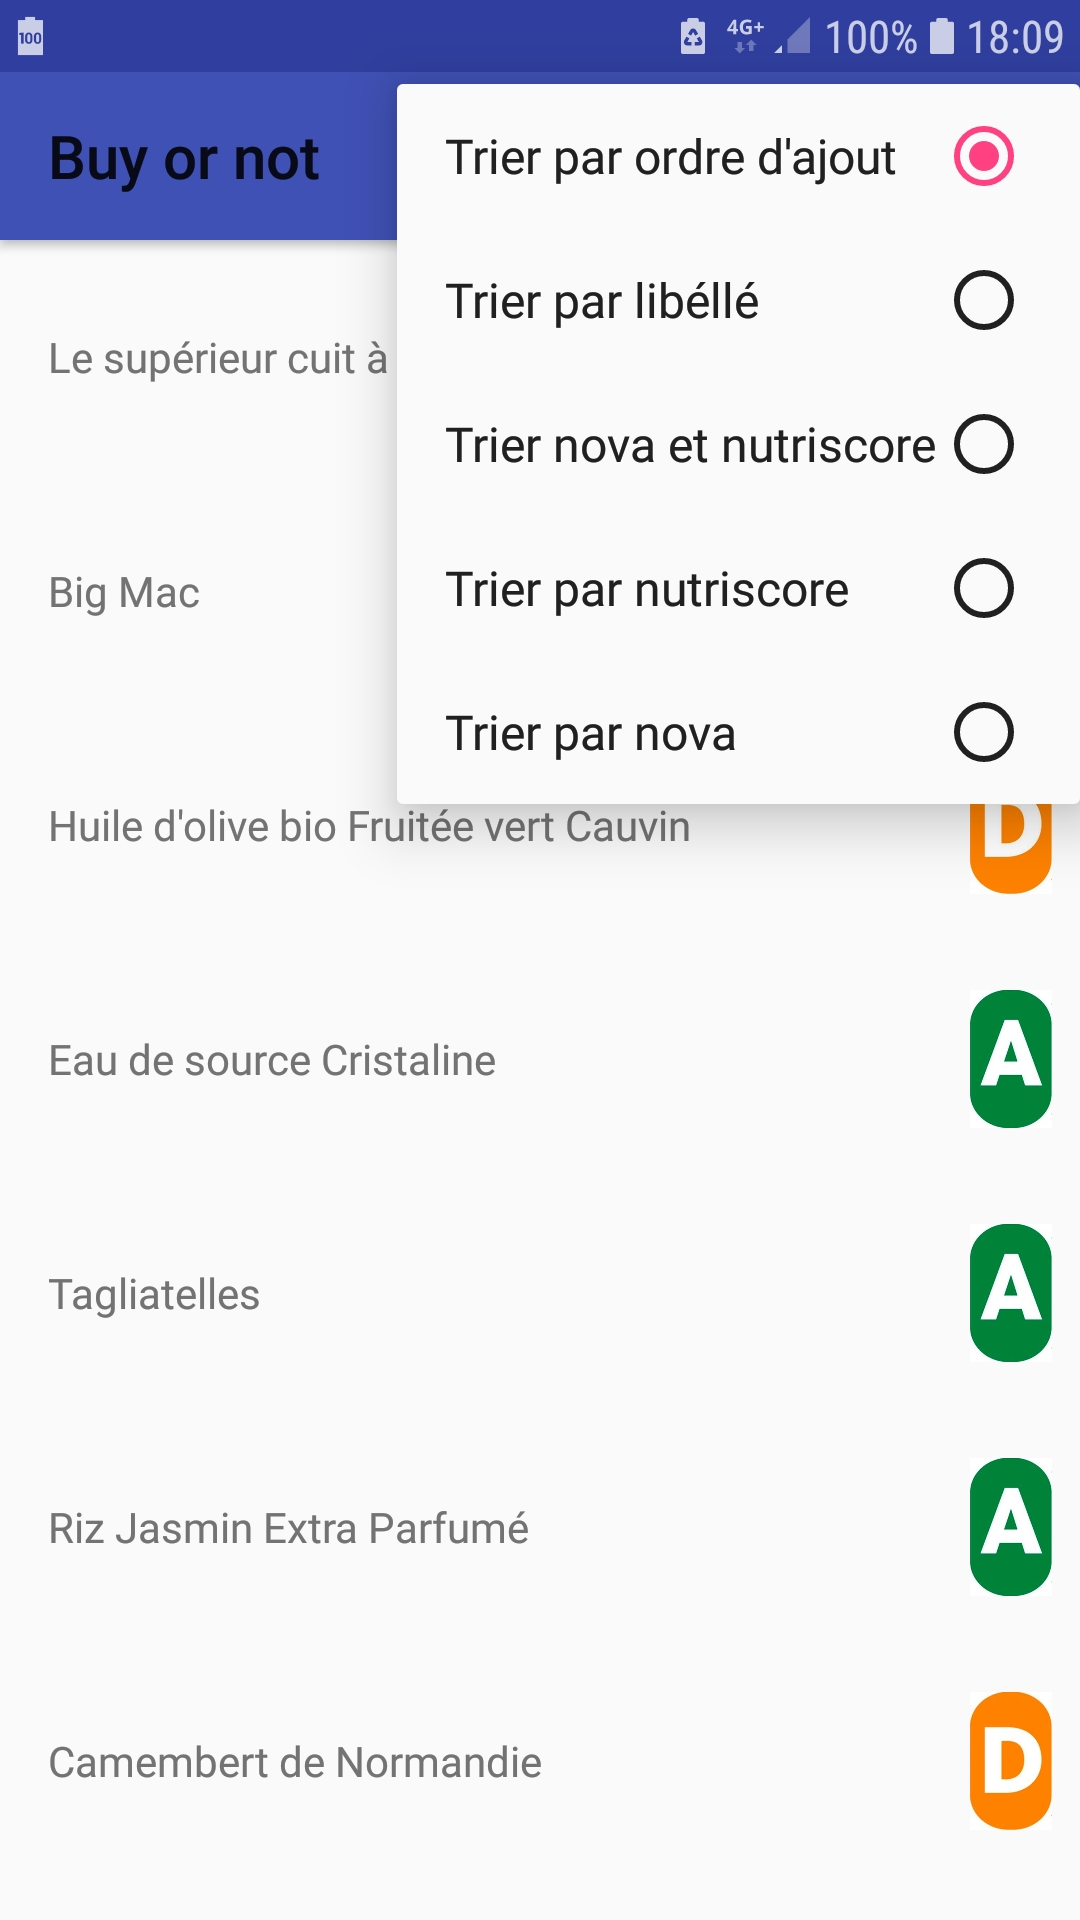
\includegraphics[width=0.5\paperwidth, height=0.3\paperheight, keepaspectratio]{img/tri.jpg}
		\captionof{figure}{Les différentes méthodes de tri}
	\end{figure}

	Ainsi lorsque l'on sélectionne le mode "Trier nova et nutriscore" on peut obtenir le résultat suivant :


	\begin{figure}[H]
		\centering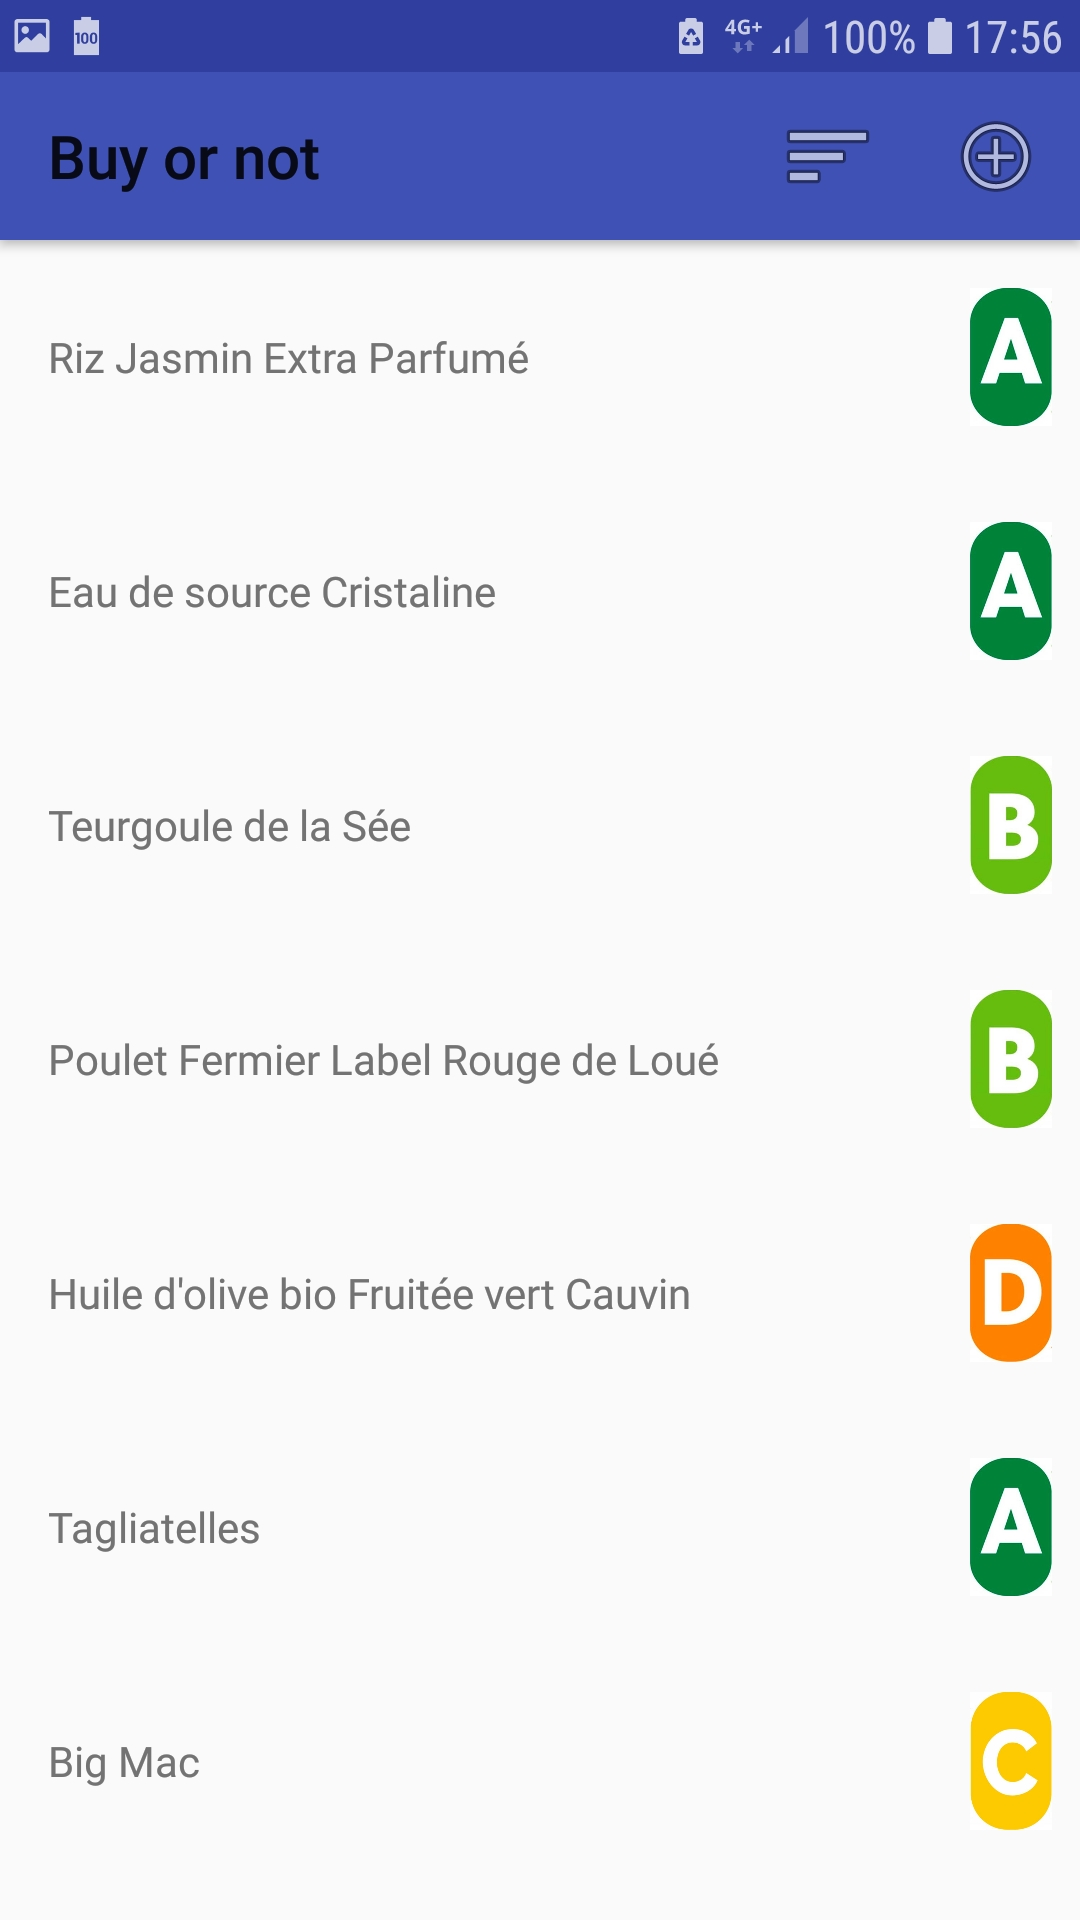
\includegraphics[width=0.5\paperwidth, height=0.3\paperheight, keepaspectratio]{img/lister_nova_nutriscore.jpg}
		\captionof{figure}{Listing des produits par score nova et nutriscore}
	\end{figure}

	\section{Consulter un produit}

	La sélection d'un produit est possible lorsque l'on clique sur un élément de la liste. On arrive alors sur la page qui sert également à modifier un produit.

	\begin{figure}[H]
		\centering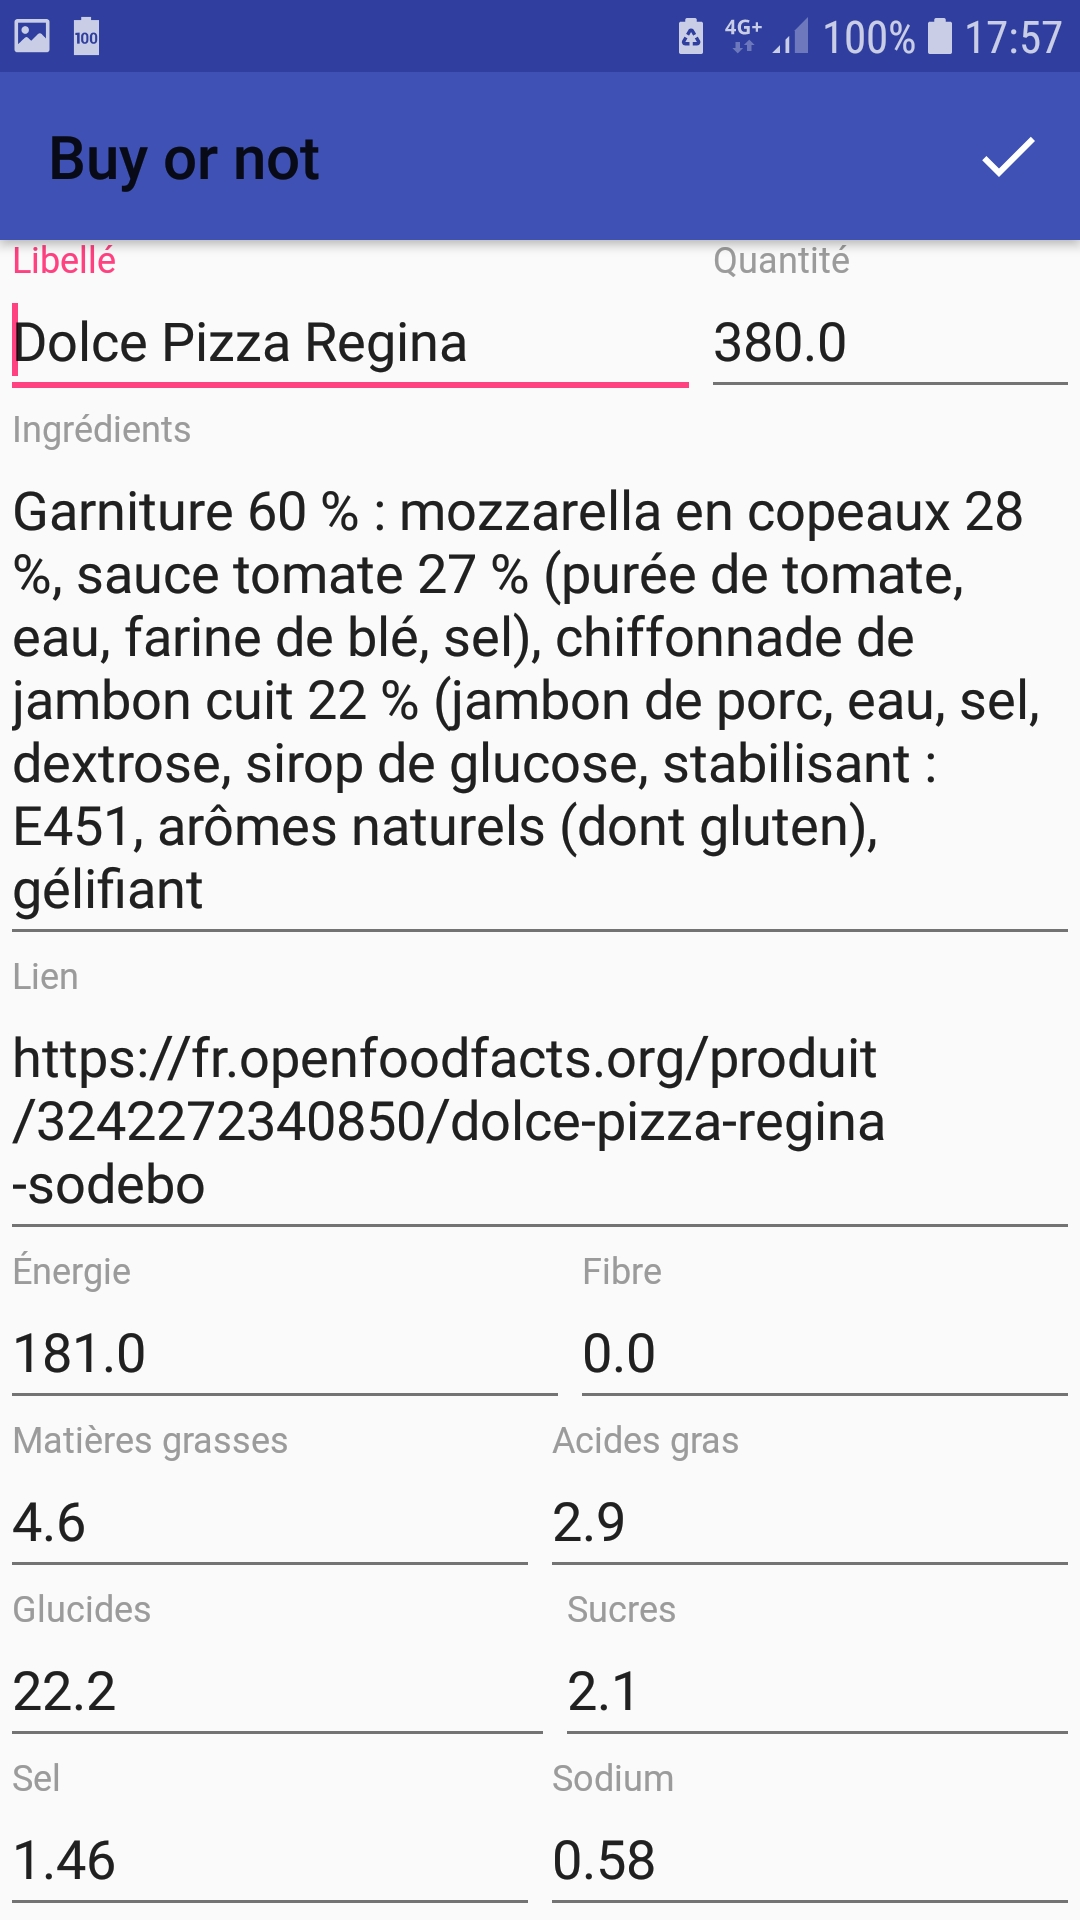
\includegraphics[width=0.5\paperwidth, height=0.3\paperheight, keepaspectratio]{img/consulter.jpg}
		\captionof{figure}{La consultation d'un produit}
	\end{figure}

	\section{Modifier un produit}

	La modification du produit est rendu possible par les différents champs disponibles sur l'écran. On peut alors valider les modifications éffectuées en cliquant sur le bouton pour valider en haut à droite de l'écran.

	Si tous les champs sont renseignés, le produit est enregistré, son nutriscore est recalculé et on retourne sur l'écran pour lister les produits.

	\section{Ajouter un produit}

	L'ajout d'un produit est possible lors du clic sur le bouton "+" en haut à droite de l'écran qui liste les produits (Voir l'image \ref{produit:consulter} \nameref{produit:consulter}). On arrive alors sur la même page que celle de modification.

	\begin{figure}[H]
		\centering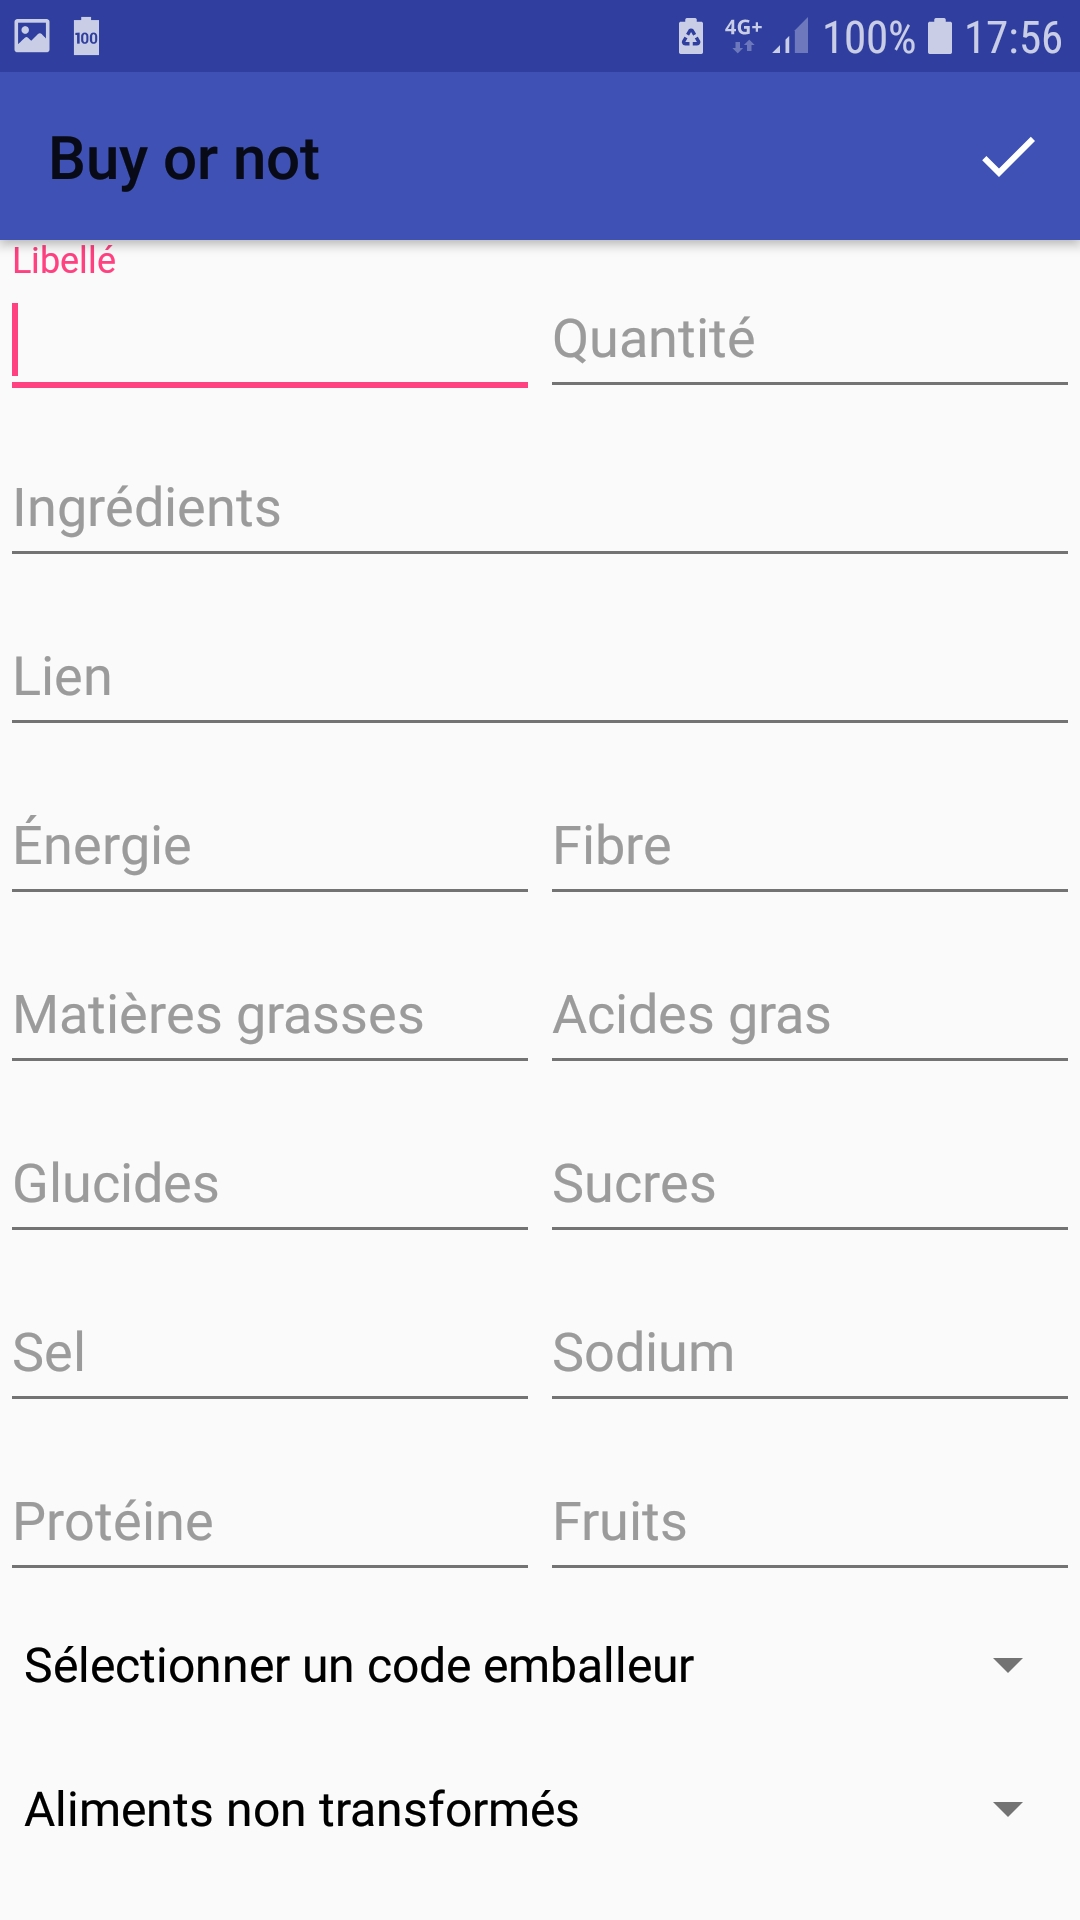
\includegraphics[width=0.5\paperwidth, height=0.3\paperheight, keepaspectratio]{img/ajout.jpg}
		\captionof{figure}{L'ajout d'un produit}
	\end{figure}

	On peut encore une fois valider le produit en cliquant en haut à droite de l'écran. Cependant, un message d'erreur apparaitra si un champs est laissé vide.

	\begin{figure}[H]
		\centering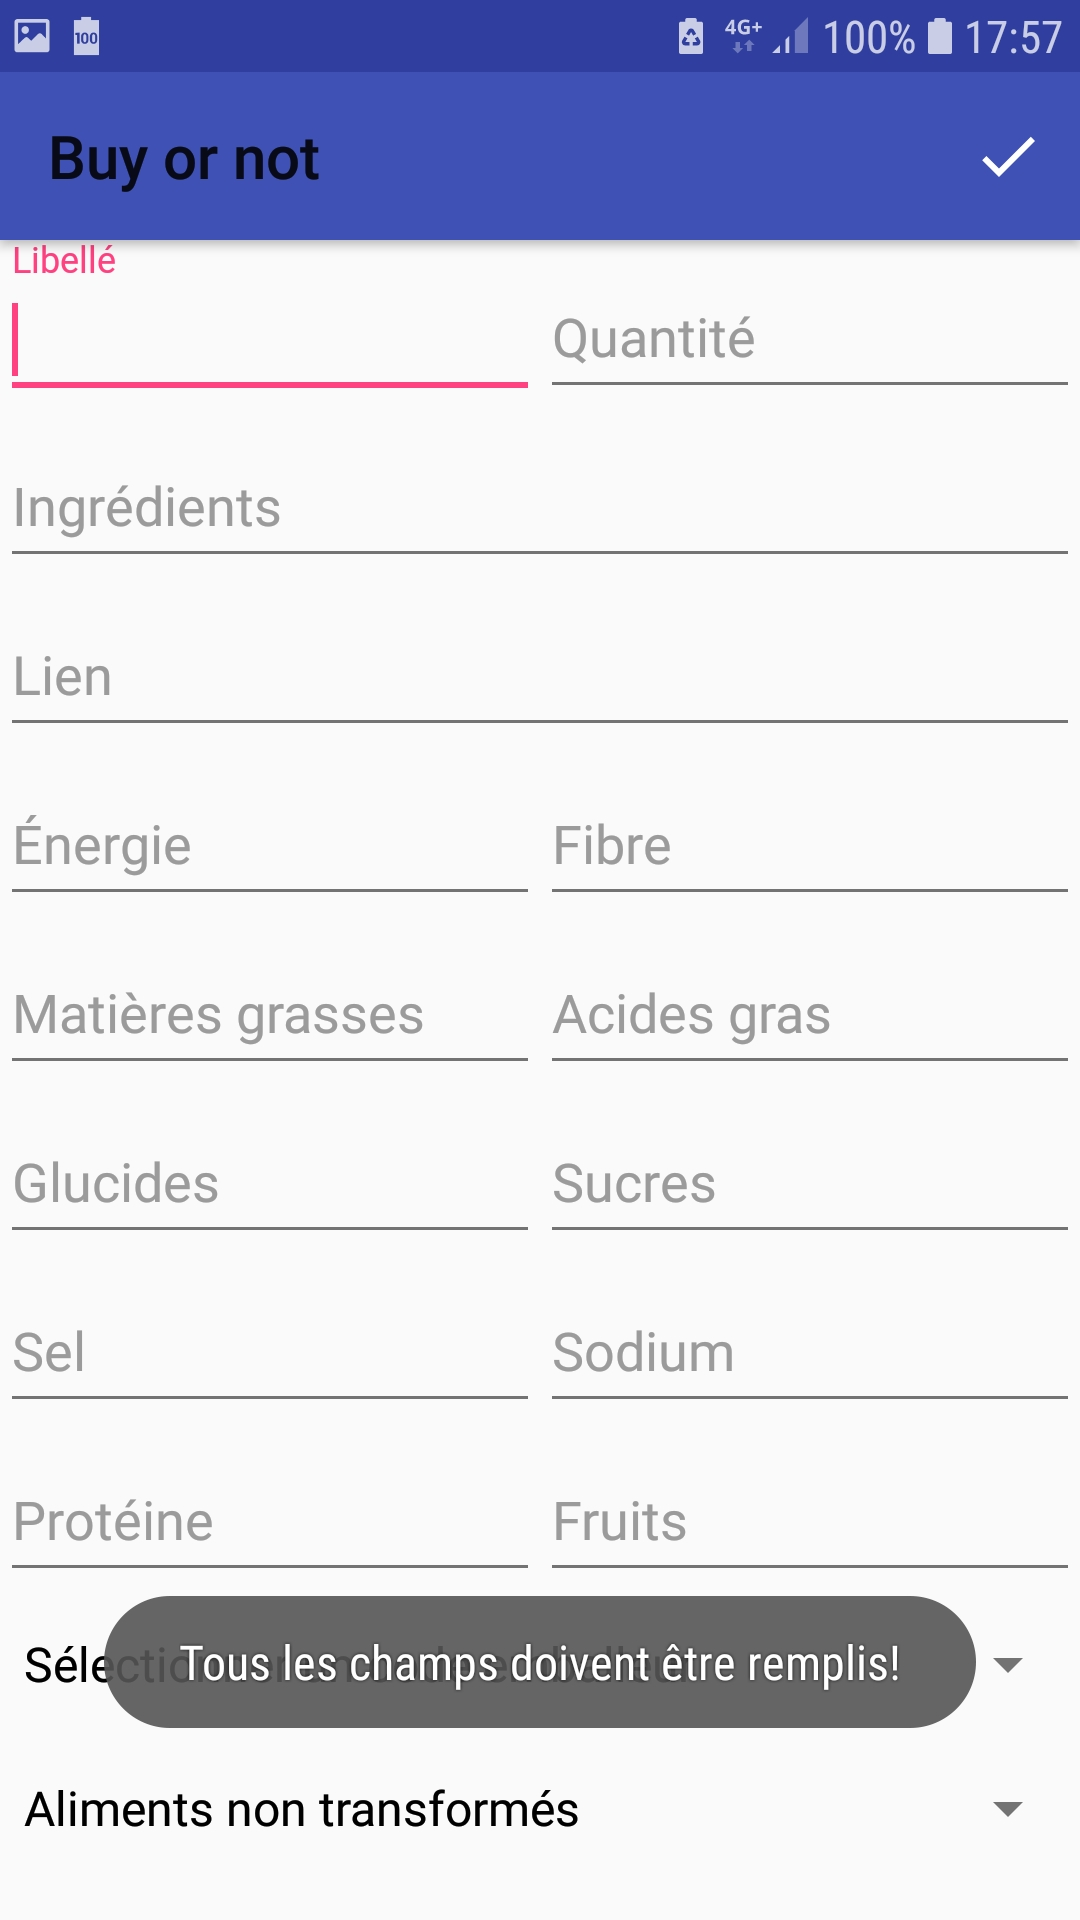
\includegraphics[width=0.5\paperwidth, height=0.3\paperheight, keepaspectratio]{img/ajout_erreur.jpg}
		\captionof{figure}{La consultation d'un produit}
	\end{figure}

	En effet, il s'agit d'une sécurité visant à vérifier que l'on possède bien les informations du produit. Si l'on ne peut pas renseigner toutes les informations, c'est surrement que l'on n'a pas le produit sous les yeux.

	Si tous les champs sont renseignés, le produit est ajouté, son nutriscore est calculé et on retourne sur l'écran pour lister les produits.

	\section{Supprimer un produit}

	La suppression d'un produit est possible lors de sa consultation. Tout en bas de la page on peut trouver un bouton supprimer.

	\begin{figure}[H]
		\centering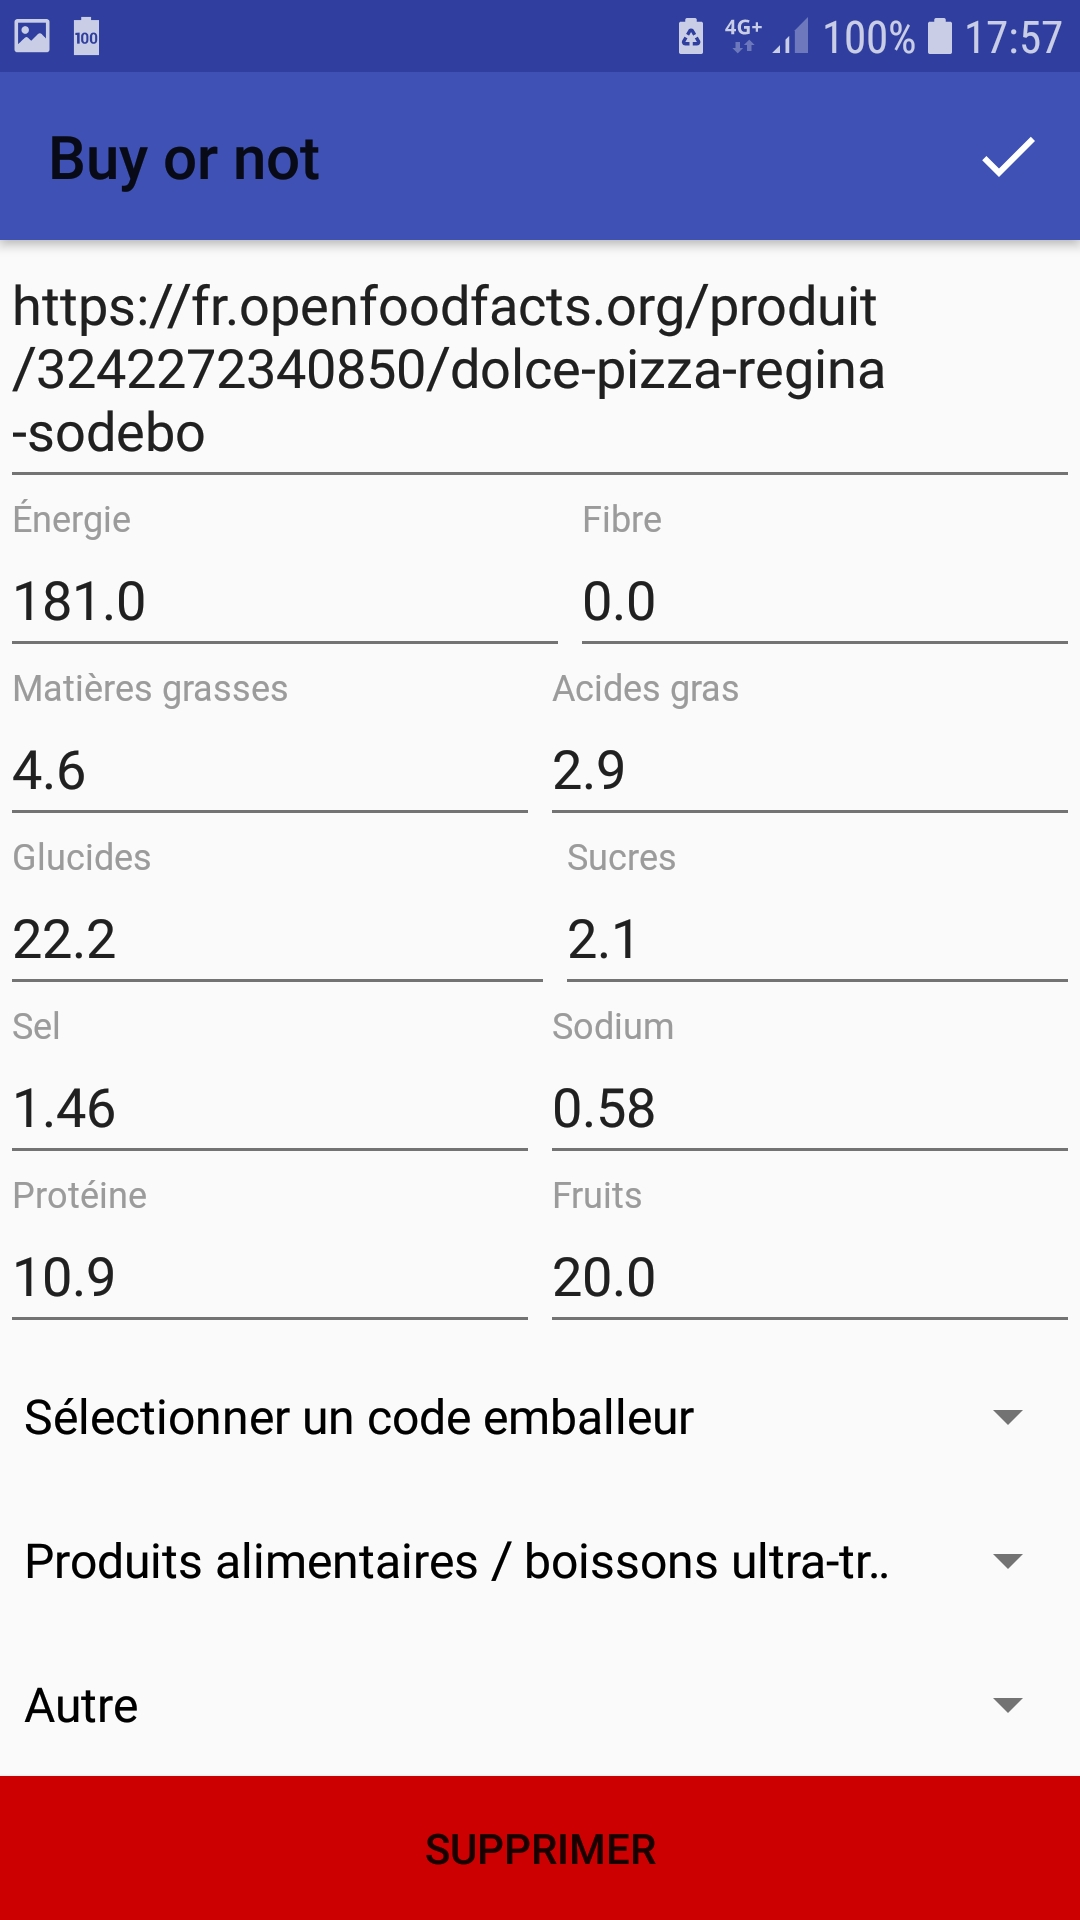
\includegraphics[width=0.5\paperwidth, height=0.3\paperheight, keepaspectratio]{img/supprimer.jpg}
		\captionof{figure}{La consultation d'un produit}
	\end{figure}

	Lors d'un clic sur ce bouton on supprime le produit et on retourne alors sur la page qui liste les produits.

	\chapter{Ressources}

	\noindent Développeuse du projet : MARTIN Justine\\
	Adresse mail : \href{mailto:justine.martin.dev@gmail.com}{justine.martin.dev@gmail.com}\\
	Github du projet : \url{https://github.com/justine-martin-study/BuyOrNot}\\
	Trello : \url{https://trello.com/b/HCXYRgZp/buy-or-not}

\end{document}
